\subsection{University of London}
\label{sec:london}

Para esta medición se eligió la Universidad de Londres (King's College, the London School of Economics and Political Science, etc), ubicada en Londres, Inglaterra. El destino propiamente dicho es \emph{'london.ac.uk'}. Se esperaría encontrar dos tramos transatlánticos: Argentina-Miami y uno transatlántico, asumiendo paso intermedio por EEUU. Hicimos las mediciones varias veces en días aledaños y los resultados fueron siempre consistentes.  Midiendo de a 30 iteraciones por TTL observamos los siguientes RTTs:
\\

\begin{figure}[H]
    \centering
    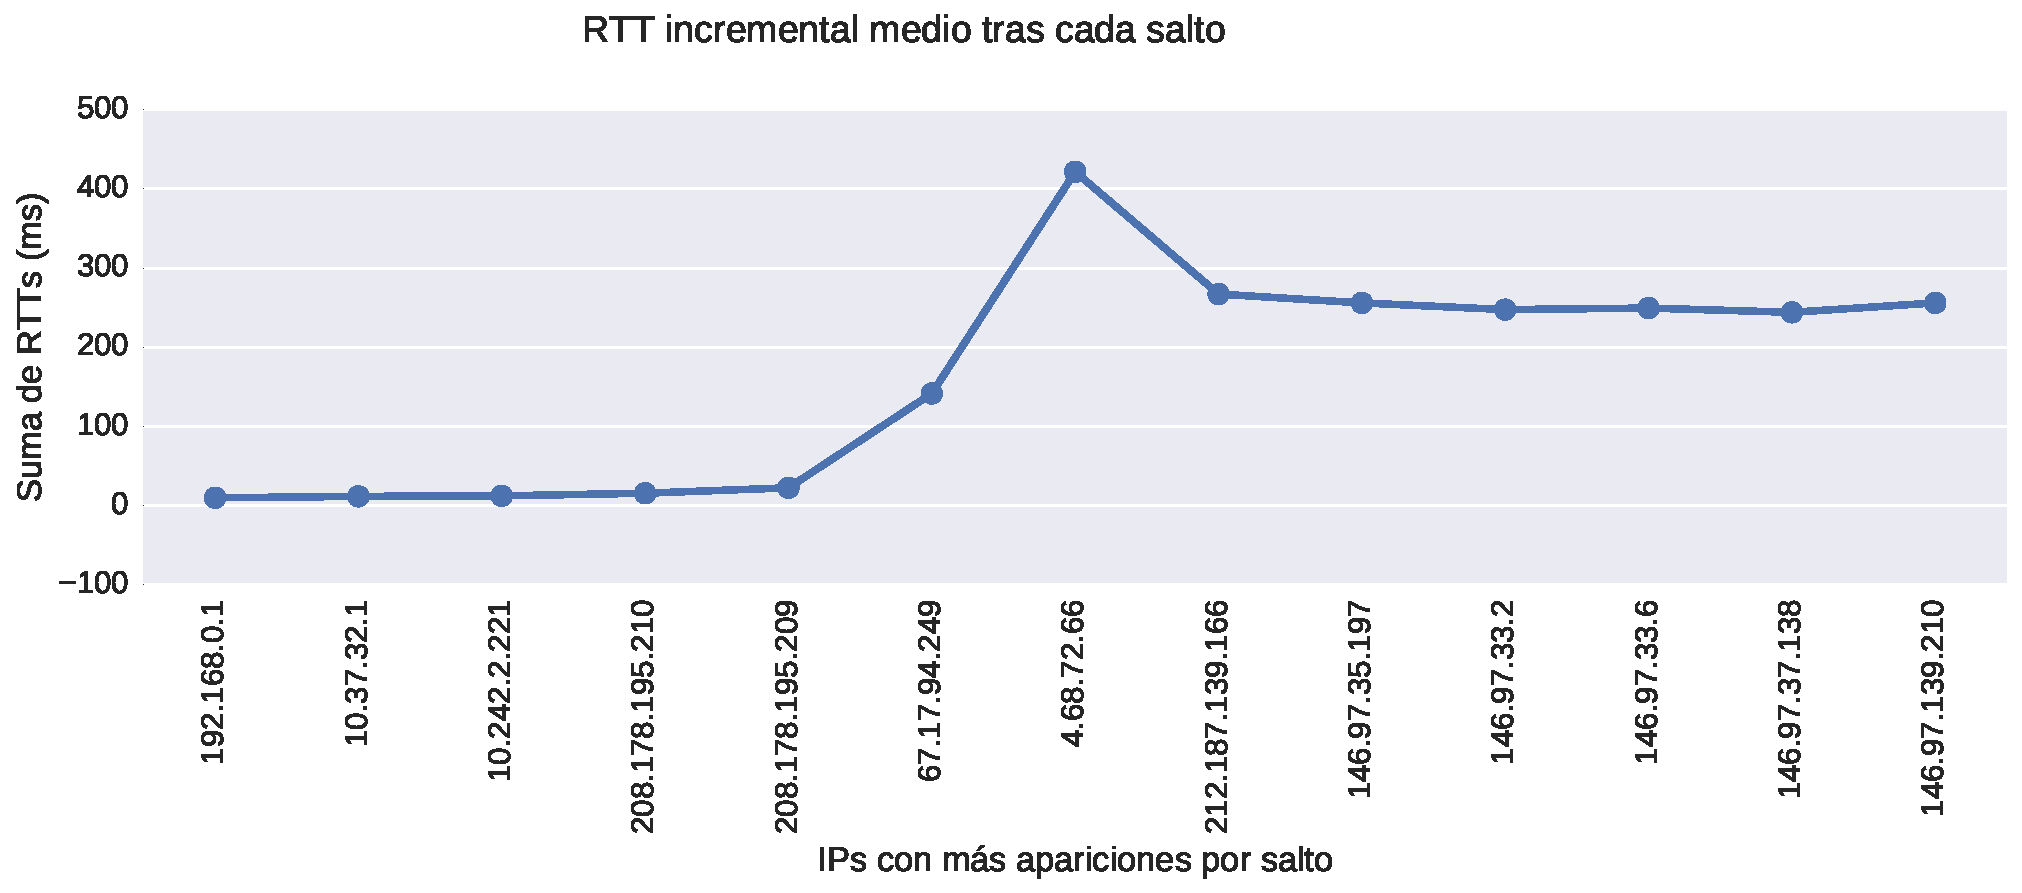
\includegraphics[width=1\textwidth, height=1\textheight, keepaspectratio]{../img/lan-incrementales}
    \caption{Comportamiento incremental de RTTs medios medidos.}
    \label{fig:lan-incrementales}
\end{figure}

Se notan dos tramos donde las diferencias entre RTTs relativos son bajas y constantes, que seguramente se corresponden al entramado interno de Buenos Aires y Londres en contraste con las rutas submarinas con mayores promedios.

\begin{figure}[H]
   \centering
       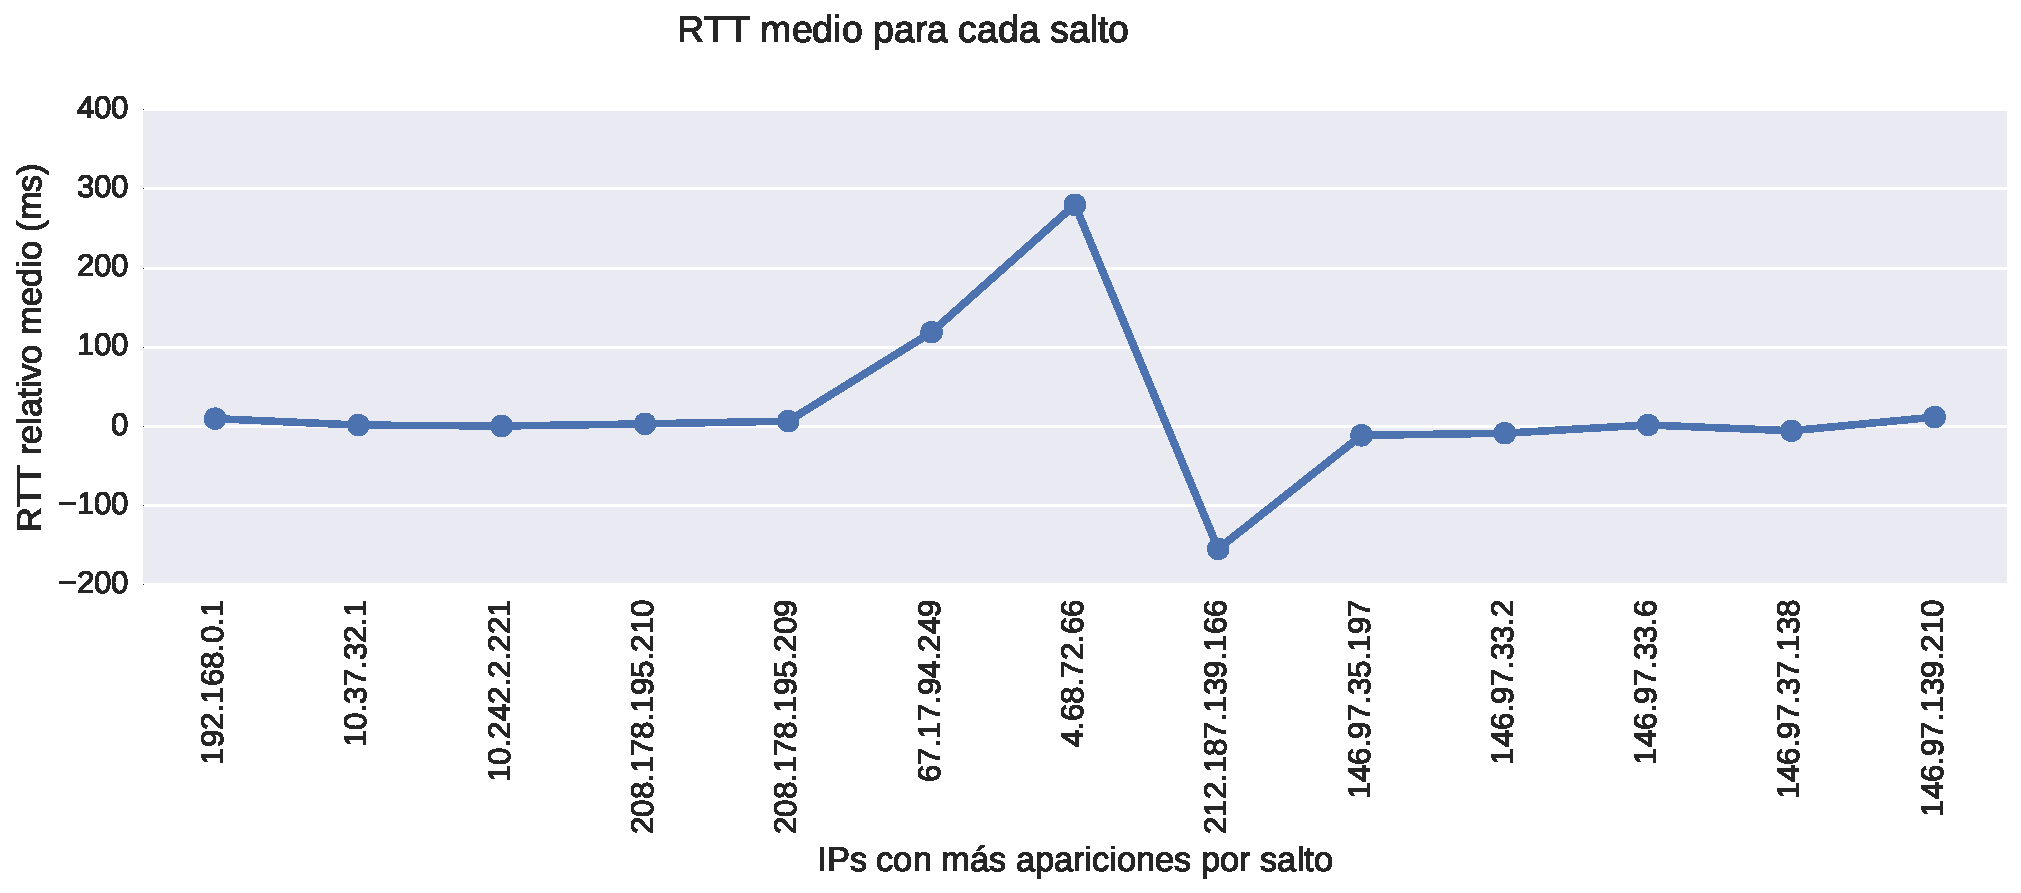
\includegraphics[width=1\textwidth, height=1\textheight, keepaspectratio]{../img/lan-rtts}
 \caption{RTTs medios medidos para una traceroute a la Universidad de Londres.}
 \label{fig:lan-rtts}
\end{figure}


Se pueden observar un gateway que conforma un pico, adjudicado a las IPs '4.68.72.66' geolocalizada en Estados Unidos con hostname \emph{'lag-9.ear1.Miami1.Level3.net'}. Podemos suponer que se trata de un gateway extremadamente cargado, posiblemente por estar en una red troncal respecto a enlaces submarinos. Este es el único nodo que cambió entre mediciones, dado que en las repeticiones posteriores y anteriores no era común su aparición, que quizás se deba a algún rebalanceo. \\


Anteriores a este salto aparecen dos nodos interesantes que son el '208.178.195.209' y '67.17.94.249', ambos adjudicados a Estados Unidos.
La '208.178.195.209' destaca porque, al igual que '208.178.195.210' tiene una latencia sospechosamente similar a las locales de Argentina. Mientras que la '67.17.94.249' presenta un gran salto respecto de su anterior en términos de RTT.

Por lo cual se especula que '208.178.195.210' y '208.178.195.209' son gateways locales, partes del backbone argentino que conecta con links internacionales. Lo cual se condice con el hostname de la última: \emph{'global-crossing-argentina-s-a.xe-0-1-0.ar3.eze1.gblx.net'}.

Esto significaría que '67.17.94.249' es el gateway del lado estadounidense del link intercontinental. \\

El nodo '212.187.139.166' es el primero adjudicado a Londres, siendo candidato a extremo británico del enlace transatlántico. Tiene promedio negativo, esto no sorprende, dado que su antecesor ('4.68.72.66') tenía un promedio muy alto.

\begin{figure}[H]
   \centering
       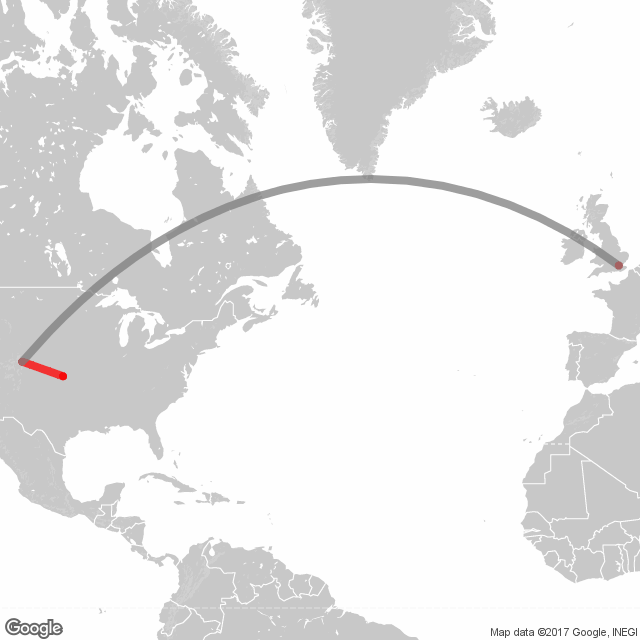
\includegraphics[width=0.5\textwidth, keepaspectratio]{../img/lan-map}
 \caption{Mapa de ubicaciones inferidas para una traceroute a la Universidad de Londres.}
 \label{fig:lan-map}
\end{figure}

Se puede notar el enlace transatlántico mencionado antes, y en rojo fuerte el gateway sobrecargado de Estados Unidos.

El traceroute presenta algo curioso, y es que todos los nodos locales a Argentina tienen asignadas IPs reservadas/privadas (192.168.0.1, 10.37.32.1, 10.242.2.221). Por lo tanto el geolocalizador solamente puede empezar a reconocer nodos a partir de las IPs estadounidenses (que, como dijimos anteriormente, las primeras están mal adjudicadas dado que probablemente estén ubicadas en el extremo argentino del enlace Argentina-Miami) significando que en el mapa el punto de origen se encuentra en dicho país. \\

Respecto al porcentaje de nodos que respondieron los \emph{requests} sucede otra anomalía: el host destino parecería no estar configurado para emitir respuestas de este tipo. Esto implica que el traceroute sigue emitiendo hasta llegar al límite preestablecido de los 30 \emph{hoops}, y no poder determinar con total seguridad en qué salto se llega al destino (y cuántos en el medio no respondieron).

Asumiendo que es el último en responder (responde por \emph{time-exceeded}, no \emph{echo-reply}), el porcentaje sería aproximadamente del \textbf{93\%} con un único nodo mudo ubicado entre '67.17.94.249' y '4.68.72.66', es decir en el backbone estadounidense.



\begin{figure}[H]
   \centering
       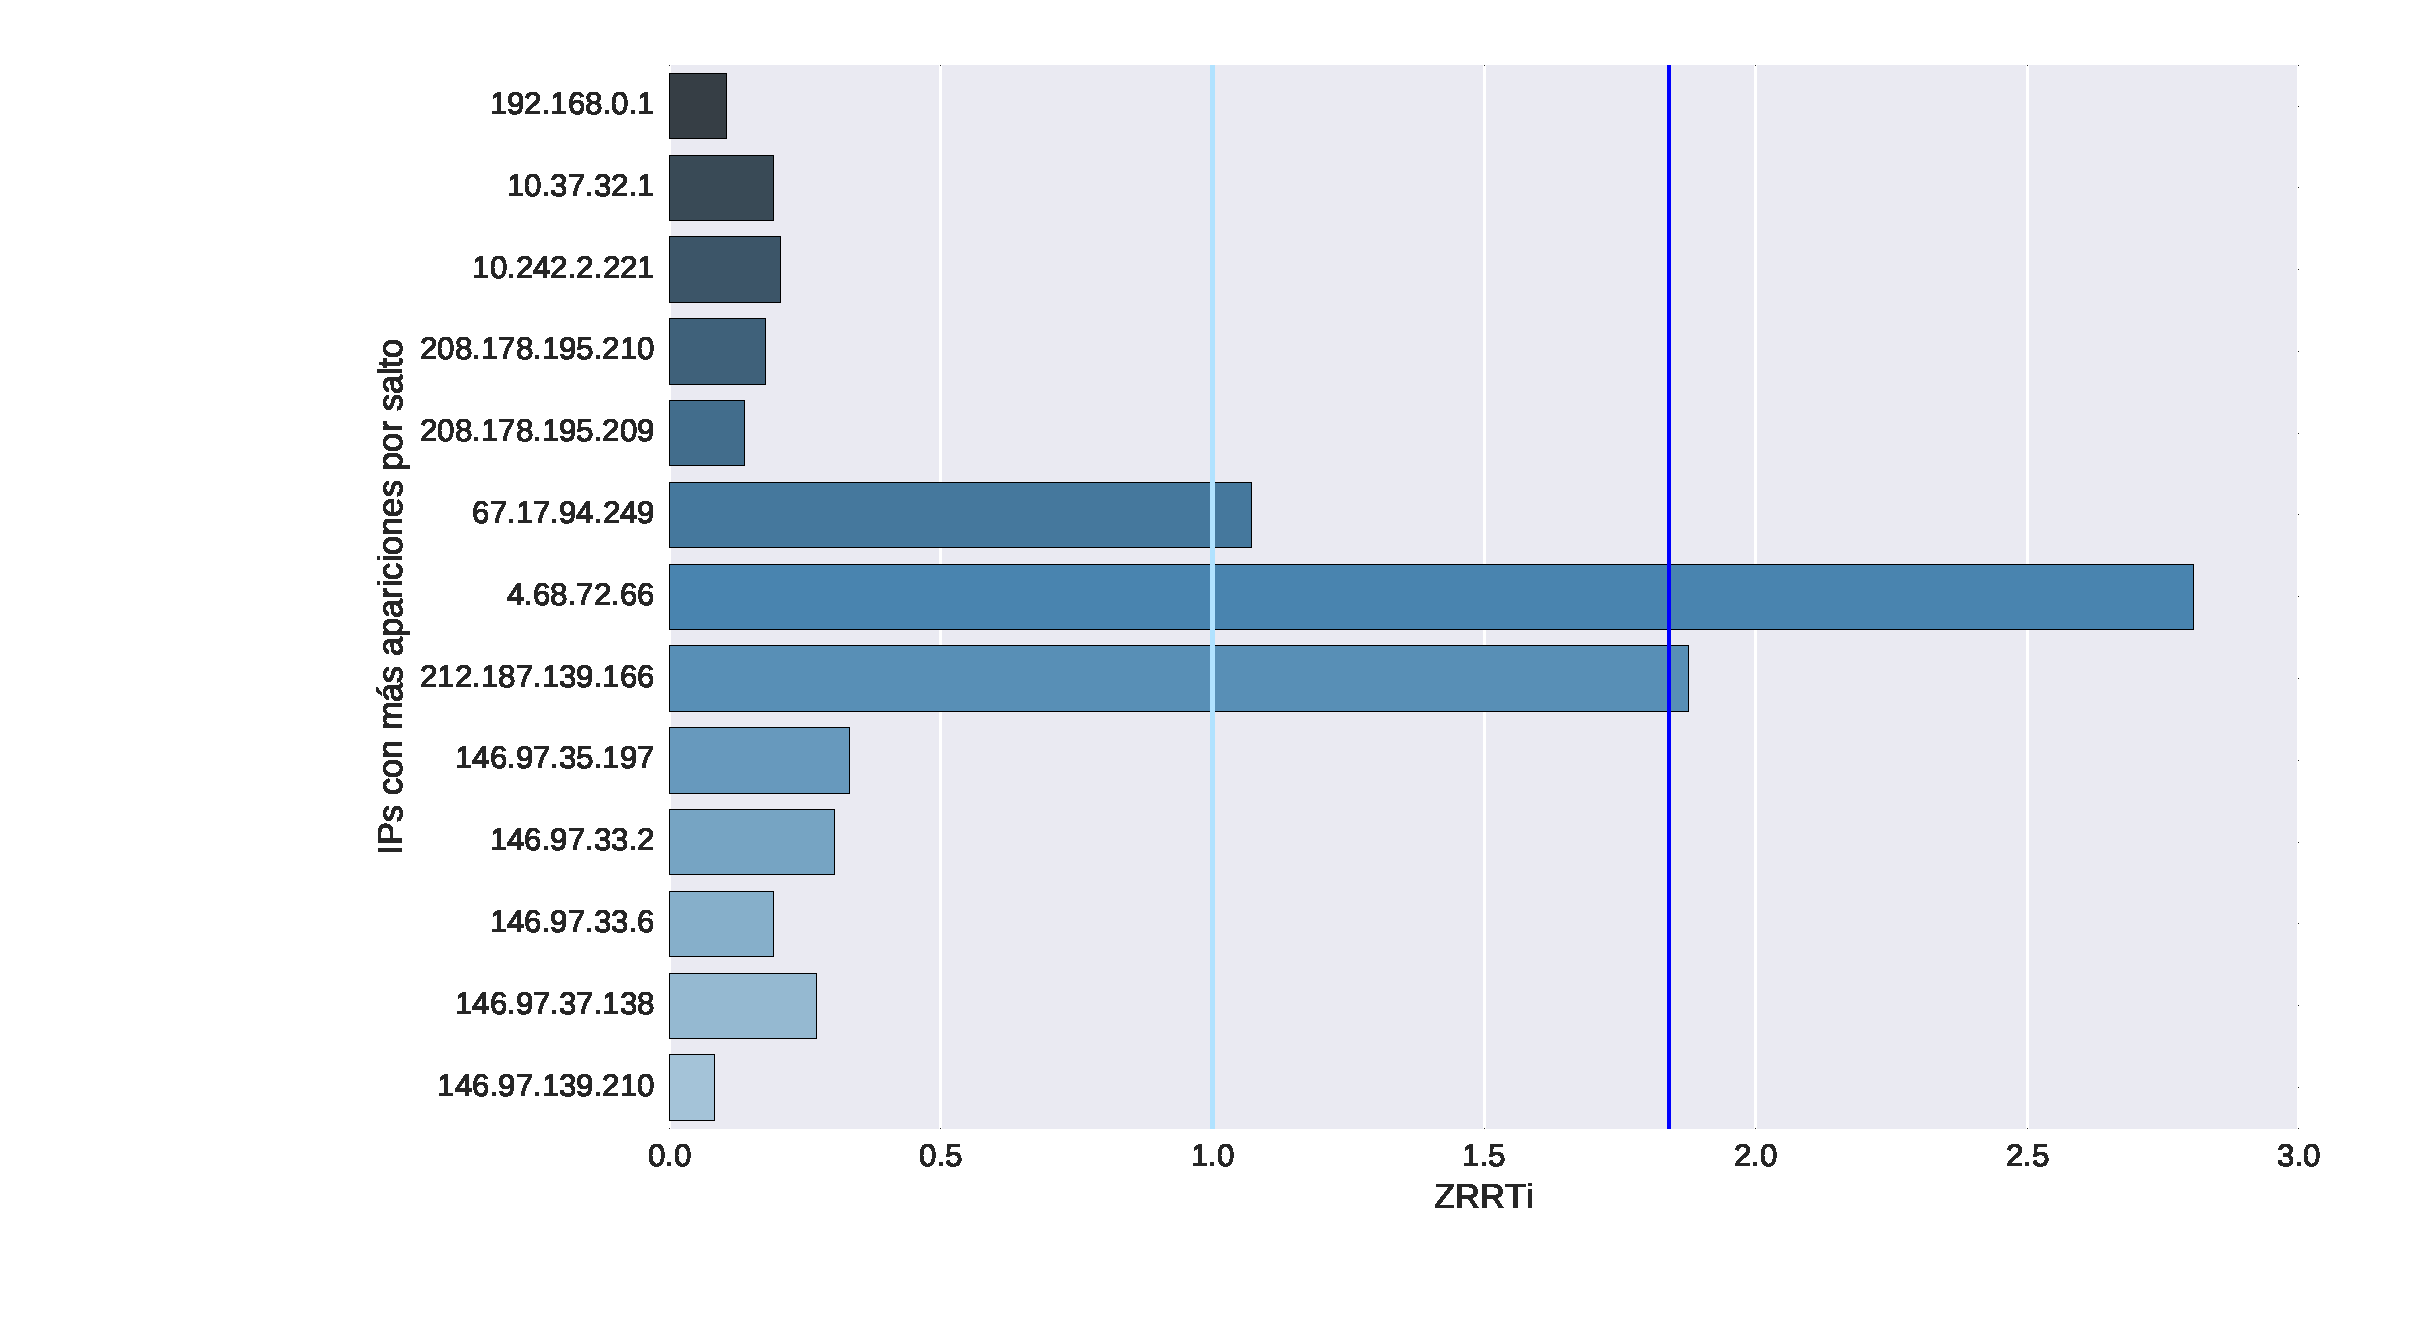
\includegraphics[width=1\textwidth, height=1\textheight, keepaspectratio]{../img/lan-zrtt}
 \caption{Outliers de la distribución ZRRTi según el método de Cimbala. En azul oscuro: valor $ZRTT_i$ correspondiente a $\tau(n)$ con $n$ el largo de ruta y un alfa fijo (0.05 sugerido en el paper de referencia).}
 \label{fig:lan-zrtt}
\end{figure}

En la figura \ref{fig:lan-zrtt} se ven los outliers de la muestra. Respecto del umbral de la tabla $\tau$, se distinguen los nodos del extremo británico del transatlántico y el gateway sobrecargado de EEUU, que no es extremo intercontinental pero sí presentó muchísima latencia. \\

El otro extremo intercontinental que falta, el de Argentina-Miami aparece con el umbral $Z=1$ (es decir aquellos que están por encima de la desviación estándar normalizada) junto a los dos anteriores, pasando de un falso negativo y un falso positivo, a un único error del tipo falso positivo para el nodo en sobrecarga. Por lo tanto el modelado de la distribución es relativamente exitoso para encontrar dichos tramos, aunque el gateway más destacado no sea un tramo intercontinental.
